\documentclass{sockitguide}

\begin{document}

\sockittitle{Getting Started on Arrow SoCKit}

This guide will help you get up and running on an Arrow SoCKit board,
by installing Linux and programming the FPGA with a simple piece of
hardware. This guide is oriented towards getting things working
quickly, making heavy use of prepared material that should have come
with this guide. For more detailed information, please read the other
guides that came with these materials.

To complete this guide you will need
\begin{itemize}
\item an Arrow SoCKit board, with associated cables,
\item a MicroSD card with at least \SI{1}{\gibi\byte} of storage,
\item an SD card reader,
\item an Ethernet cable with an internet connection.
\end{itemize}

\section{Installing Linux}

We will be installing a copy of \fnurl{Debian
  Linux}{https://www.debian.org/} on to the SD card, and using that to
boot the SoCKit board into Linux. If you have ever used a Raspberry Pi
or other single-board computer, this process will be similar.

First, we need to configure the board to allow the hard processor
(soon to be running Linux) to be able to configure the FPGA
directly. To do that, find the small set of switches on the back of
the board labeled \texttt{MSEL}, and move the switches into place as indicated in \Cref{fig:msel}.

\begin{figure}[h]
  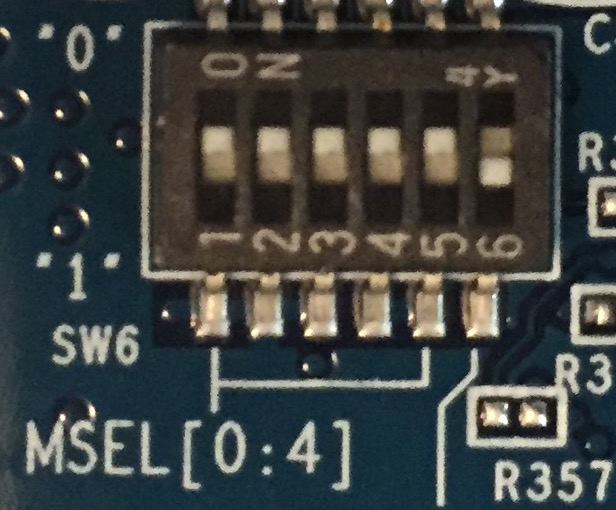
\includegraphics[width=4cm]{figures/msel.png}
  \caption{\texttt{MSEL} configuration on back of board. Move switches
    \numrange{1}{5} towards the \texttt{ON} label, and move switch
    \num{6} away.}
  \label{fig:msel}
\end{figure}

Alongside this guide, there should be a large file named
\directory{debian.img.bz2}. Please download this file now. We are
going to write this file to the MicroSD card using a program named
\fnurl{Etcher}{https://etcher.io/}, which simplifies the process. If
you already know how to write SD card images and would rather do it
differently, feel free.

Launch Etcher, and as the first step, select the
\directory{debian.img.bz2} file you downloaded earlier. Then, select the
SD card reader you are using as the destination drive. \textit{Be
  careful to choose correctly!} Writing to the wrong drive will
destroy any data already on that drive.

Once you have set the image file and destination drive (see
\Cref{fig:etcher}), click the \menu{Flash!} button to begin writing
to the SD card. This can take some time.

\begin{figure}
  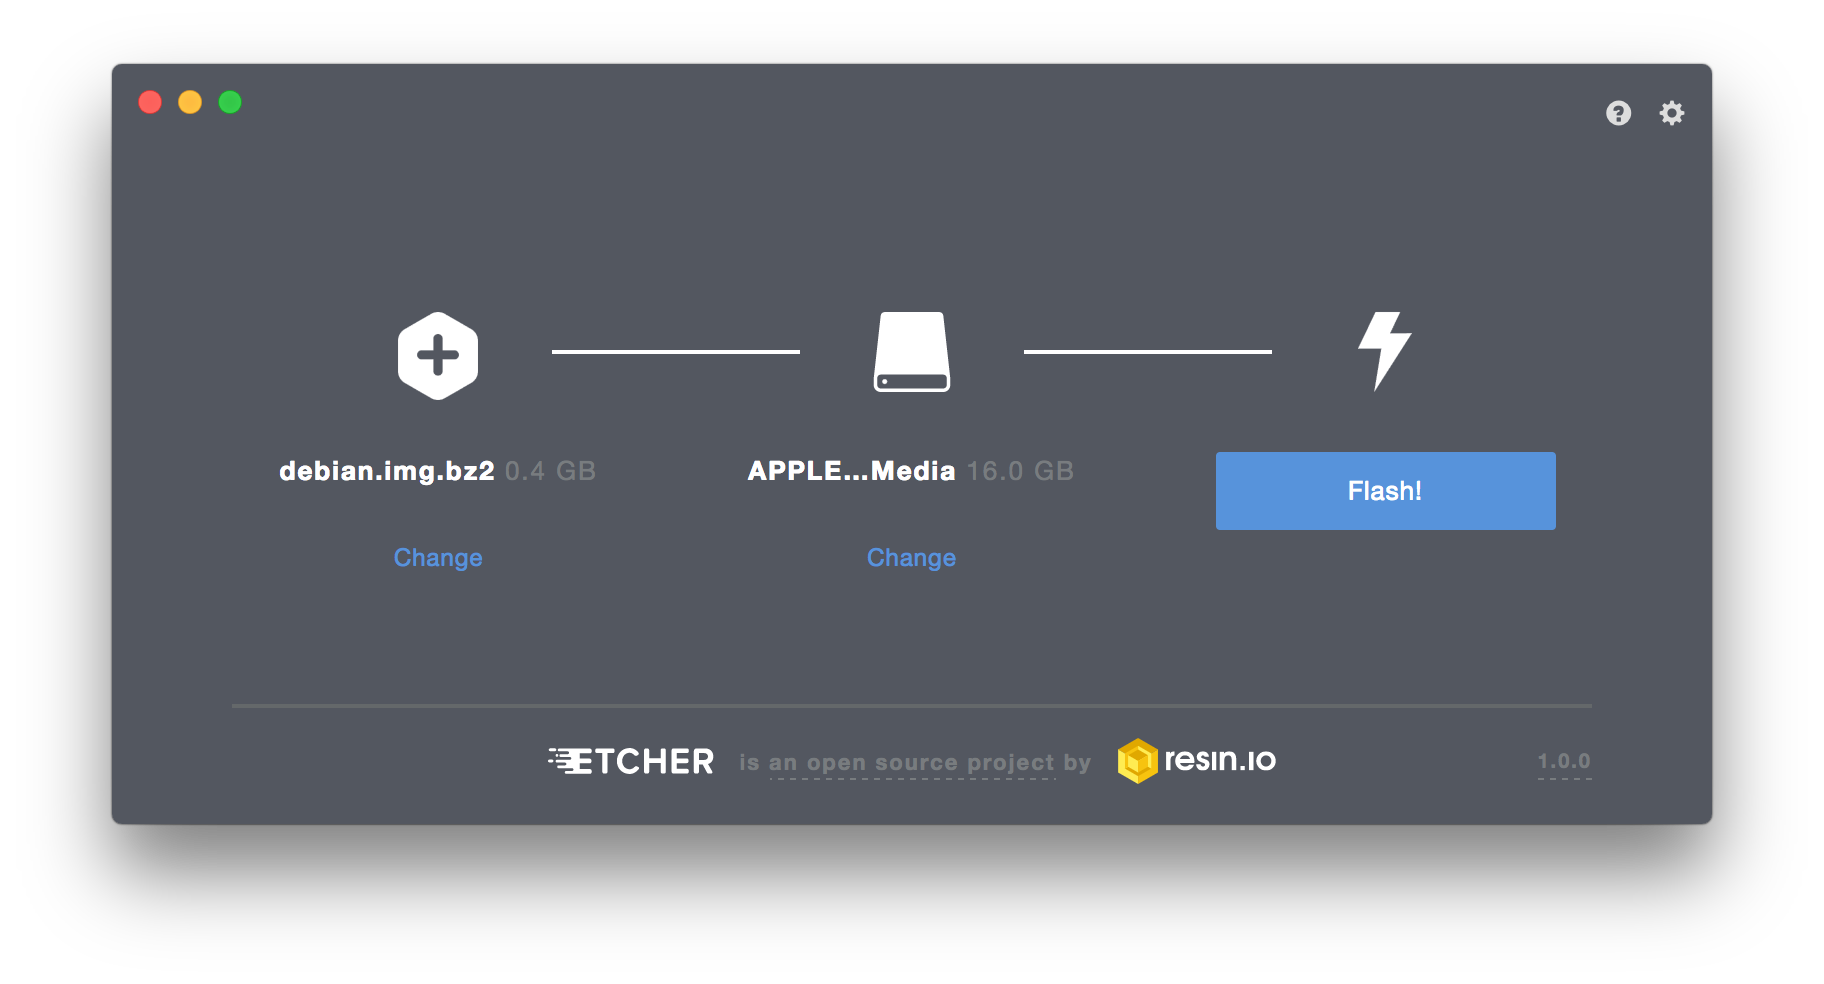
\includegraphics[width=9cm]{figures/etcher.png}
  \caption{Example of a properly configured Etcher window, ready to write.}
  \label{fig:etcher}
\end{figure}

Once Etcher is done, remove your SD card and push it into the MicroSD
card slot underneath the SoCKit board. Before turning the SoCKit on,
connect it to power with the supplied cable, and connect the Ethernet
cable that you know provides an internet connection.

\section{Connecting to Serial Console}

The SoCKit has \num{3} USB ports:
\begin{itemize}
\item a USB-Blaster II port,
\item an HPS-USB port,
\item a UART to USB port.
\end{itemize}
They are labeled on the board.

Connect one end of the supplied USB cable to the UART to USB port, and
the other end to your computer. We will use this cable to view the
serial console presented by Linux when it boots. How we do this will
depend on what operating system you are currently using.

\subsection{Windows}

When you plug in the SoCKit UART to USB cable, it creates a new serial
console on your computer, even when the SoCKit is off. To use this
console, you need to install the \fnurl{FTDI VCP
  drivers}{http://www.ftdichip.com/Drivers/VCP.htm}, and also download
\fnurl{PuTTY}{https://www.chiark.greenend.org.uk/~sgtatham/putty/latest.html}
for Windows.

Once you have these, you can discover the name of this serial console
by opening the ``Windows Device Manager''. The console should be
listed under ``\textit{Ports (COM \& LPT)}'' as ``\textit{USB Serial
  Port}''. You should note down the COM port it uses, such as
\texttt{COM4}. See \Cref{fig:devman} for an example.

\begin{figure}
  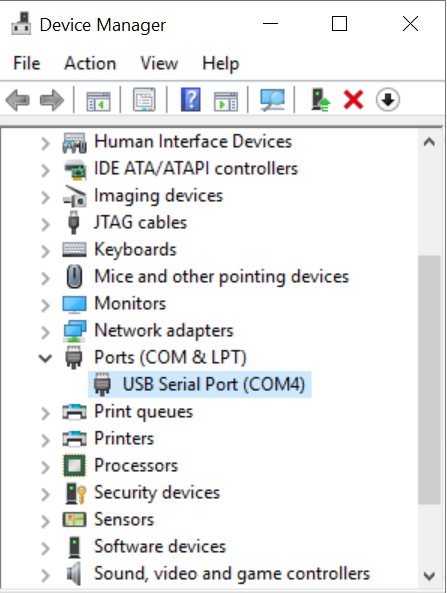
\includegraphics[width=4cm]{figures/devicemanager.png}
  \caption{Windows Device Manager, showing the ``USB Serial Port''
    named \texttt{COM4} selected.}
  \label{fig:devman}
\end{figure}

Now, launch PuTTY, and in the configuration window that pops up click
the \menu{Serial} radio button, then type in your port name
(like \texttt{COM4}) into the \menu{Serial line} field. Then,
type \num{115200} into the \menu{Speed} field. It should look
something like \Cref{fig:putty}. Finally, click the \menu{Open}
button.

\begin{figure}
  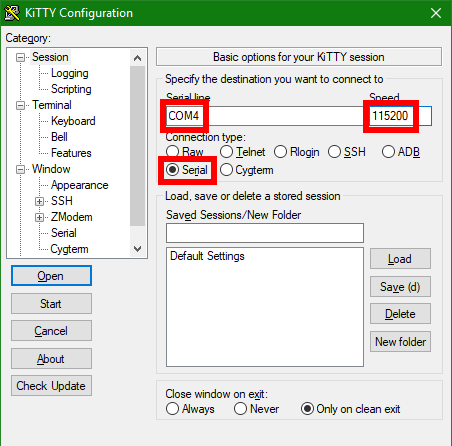
\includegraphics[width=6cm]{figures/putty.png}
  \caption{Example configuration for PuTTY to talk to the serial console.}
  \label{fig:putty}
\end{figure}

You should see a blank screen, but that will shortly fill with text
once we turn the SoCKit on.

\subsection{Linux or MacOS}

When you plug in the SoCKit UART to USB cable, it creates a new serial
console on your computer, even when the SoCKit is off. Open a terminal
window and determine what that new serial console is called by
running:
\begin{minted}{console}
  $ ls /dev/tty.usb*
  $ ls /dev/ttyUSB*
\end{minted}

Look for these commands to print out a name like
\texttt{/dev/tty.usbserial-AH03P0DR} or \texttt{/dev/ttyUSB0}; this is
your serial console name. To connect to it, we can use \fnurl{GNU
  Screen}{https://www.gnu.org/software/screen/}:
\begin{minted}{console}
  $ screen /dev/ttyUSB0 115200
\end{minted}
(Use your own console name instead of \texttt{/dev/ttyUSB0}.)

You should see a blank screen, but that will shortly fill with text
once we turn the SoCKit on. When you wish to exit the serial console,
hit \keys{\ctrl + A} then \keys{K}, followed by \keys{Y} to confirm.

\section{Booting Linux}

Now that you have the serial console visible, you can turn on the
SoCKit by pushing the big red button on the top of the board. You
should first see some text from U-boot, then a countdown, and then
eventually a series of messages that looks like \Cref{fig:boot}. If
you see these \texttt{OK} statuses, then everything is working! If
not, go back and see if you missed something, or contact me.

\begin{figure}
  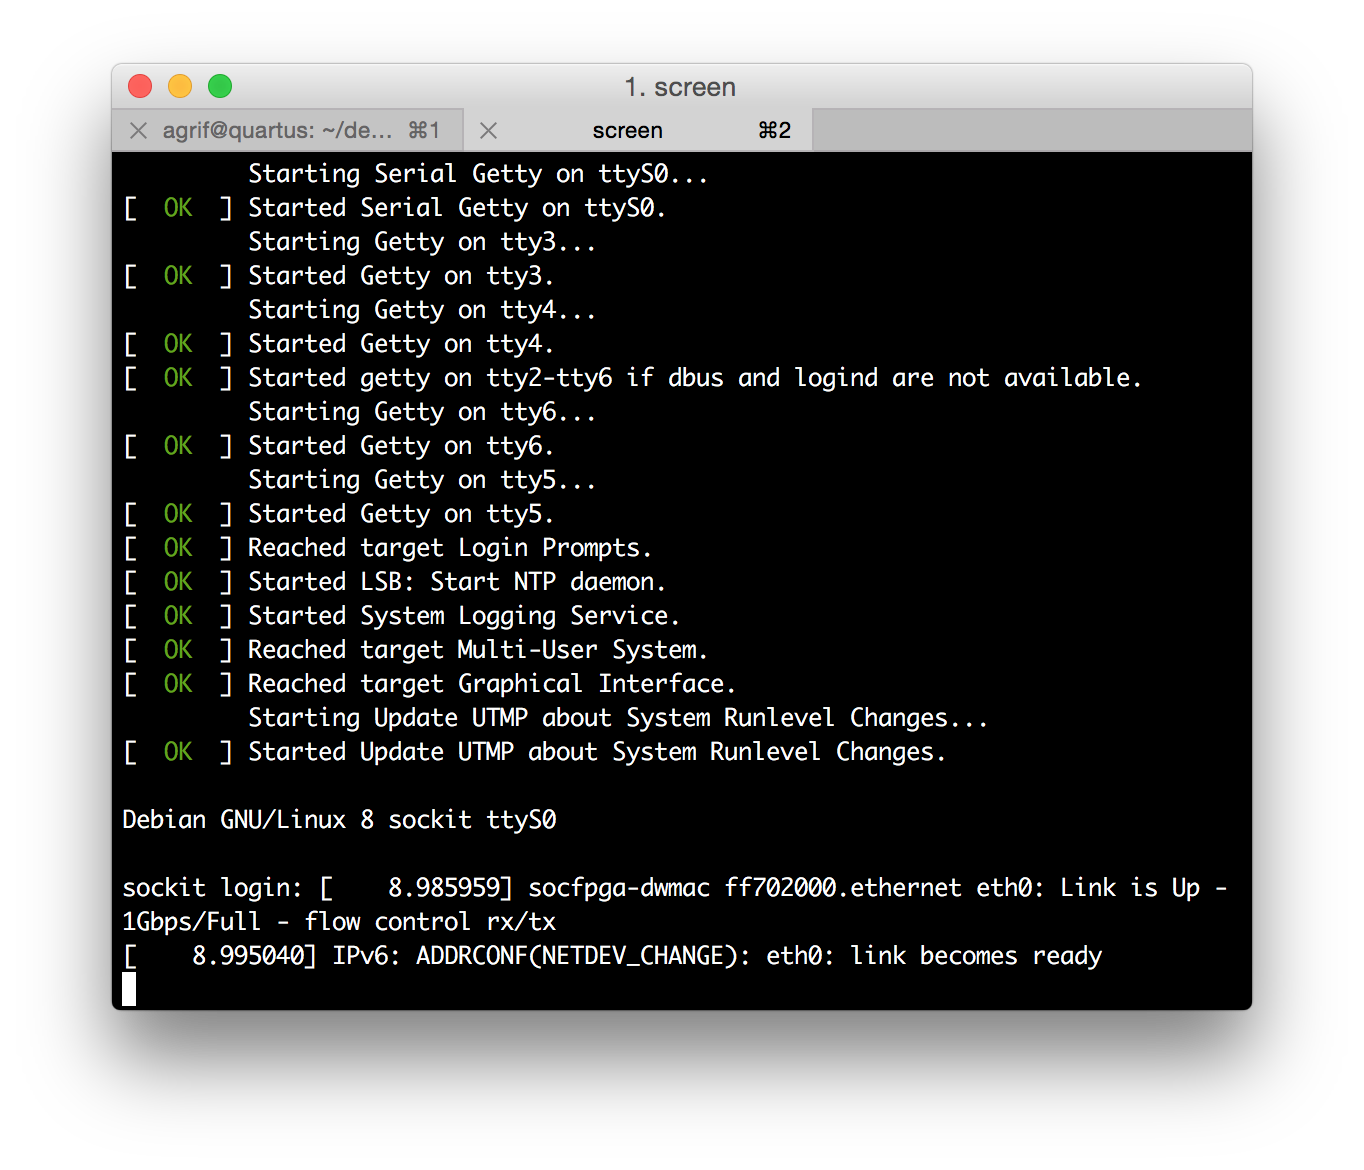
\includegraphics[width=9cm]{figures/boot.png}
  \caption{A working, booted Linux on the SoCKit serial console.}
  \label{fig:boot}
\end{figure}

Now that you have a login prompt, you can log in with the username
\texttt{sockit} and password \texttt{arrow}.

\section{Connecting over SSH}

Setting up the serial console every time can be awkward, but the
version of Linux we installed supports
\fnurl{SSH}{https://en.wikipedia.org/wiki/Secure_Shell}, which lets
you connect to the board over the network, provided your computer is
on the same network as the SoCKit board.

To connect over SSH instead, we need to know the IP address of the
board. This can change every time the board starts up, but we can read
it over the serial console:
\begin{minted}{console}
  $ hostname -I
  128.146.33.233
\end{minted}

In Windows, you can paste this address in to the PuTTY field for
\menu{Host Name}, and PuTTY will directly connect to your board over the
network, without using USB.

On Linux or MacOS, you can log in to your board over SSH with the
username \texttt{sockit} on the command line with:
\begin{minted}{console}
  $ ssh sockit@<put ip address here>
\end{minted}

Once connected, you can close the session by running \texttt{exit}.

Using SSH instead of the serial console is entirely up to you, but you
may find it convenient. In particular, you can use it to transfer
files using \fnurl{WinSCP}{https://winscp.net/eng/download.php} on
Windows, or the \fnurl{\texttt{scp}}{https://linux.die.net/man/1/scp}
command on Linux or MacOS.

\section{Resizing the Disk}

The SD card image you wrote was made to be small enough to download,
but chances are that your actual SD card is much larger. We can expand
the amount of space Linux uses on it so we won't run in to space
issues later:
\begin{minted}{console}
  $ sudo fdisk /dev/mmcblk0
  [sudo] password for sockit: <type password>
  Welcome to fdisk (util-linux 2.25.2).
  ...
  Command (m for help): d
  Partition number (1-3, default 3): 2

  Partition 2 has been deleted.

  Command (m for help): n
  Partition type
    p  primary (2 primary, 0 extended, 2 free)
    e  extended (container for logical partitions)
  Select (default p): p
  Partition number (2, 4, default 2): 2
  First sector (...): <hit enter>
  Last sector, +sectors, or +size: <hit enter>

  ...

  Command (m for help): wq
\end{minted}

After running through these commands, \texttt{fdisk} will complain
about re-reading the partition table; this is normal. To force Linux
to recognize the new space, we need to turn the board off and then
on. We can tell Linux to do that with:
\begin{minted}{console}
  $ sudo reboot
\end{minted}

When the board comes back online, log in again and finally run:
\begin{minted}{console}
  $ sudo resize2fs /dev/mmcblk0p2
\end{minted}

Now Linux is using your entire SD card. You can verify this by running:
\begin{minted}{console}
  $ df -h /
\end{minted}

\section{Building the Example}

Alongside this guide is a file named \directory{example.zip}, which
contains an example Quartus project for use with the SoCKit
board. Please download this, extract it, and open
\directory{example.qpf} in Quartus.

This project contains two custom IP cores, the \fnurl{Sampler and
  Player}{https://github.com/agrif/sampler-player/}, which can be used
by the hard processor (in Linux) to sample time series data on the
FPGA, as well as play back data from Linux back to the FPGA. In this
example they have been connected to each other in a loopback
configuration, for testing. Finally, there is a binary counter that
displays on the LEDs on the front of the board.

Feel free to take a moment to read \directory{example.v} and to look
at the connections made in \directory{hps\_system.qsys} inside the
Qsys editor.

To build the project, open \directory{hps\_system.qsys} inside the Qsys
editor, then regenerate the system by going to \menu{Generate >
  Generate HDL..} in the top menu. The default generation settings are
fine, so just click the \menu{Generate} button. This generates the
Verilog code for the Sampler and Player modules, as well as the
interconnect to the hard processor running Linux.

Once Qsys has finished, return to Quartus to compile by going up to
the menu and clicking \menu{Processing > Start Compilation}.

Once Quartus has finished, it is possible to program the SoCKit board
using the USB-Blaster II port and USB cable, similar to other
boards. However, we will instead use the SD card and hard processor to
program the FPGA at boot time. To do this, we need to create an RBF
file by opening menu \menu{File > Convert Programming
  Files...}. Select \menu{Raw Binary File (.rbf)} as the output
programming file type, set \directory{socfpga.rbf} as the file name,
and under ``\textit{Input files to convert}'' add the
\directory{example.sof} file that Quartus just finished compiling (see
\Cref{fig:rbf}). Finally, press the \menu{Generate} button.

\begin{figure}
  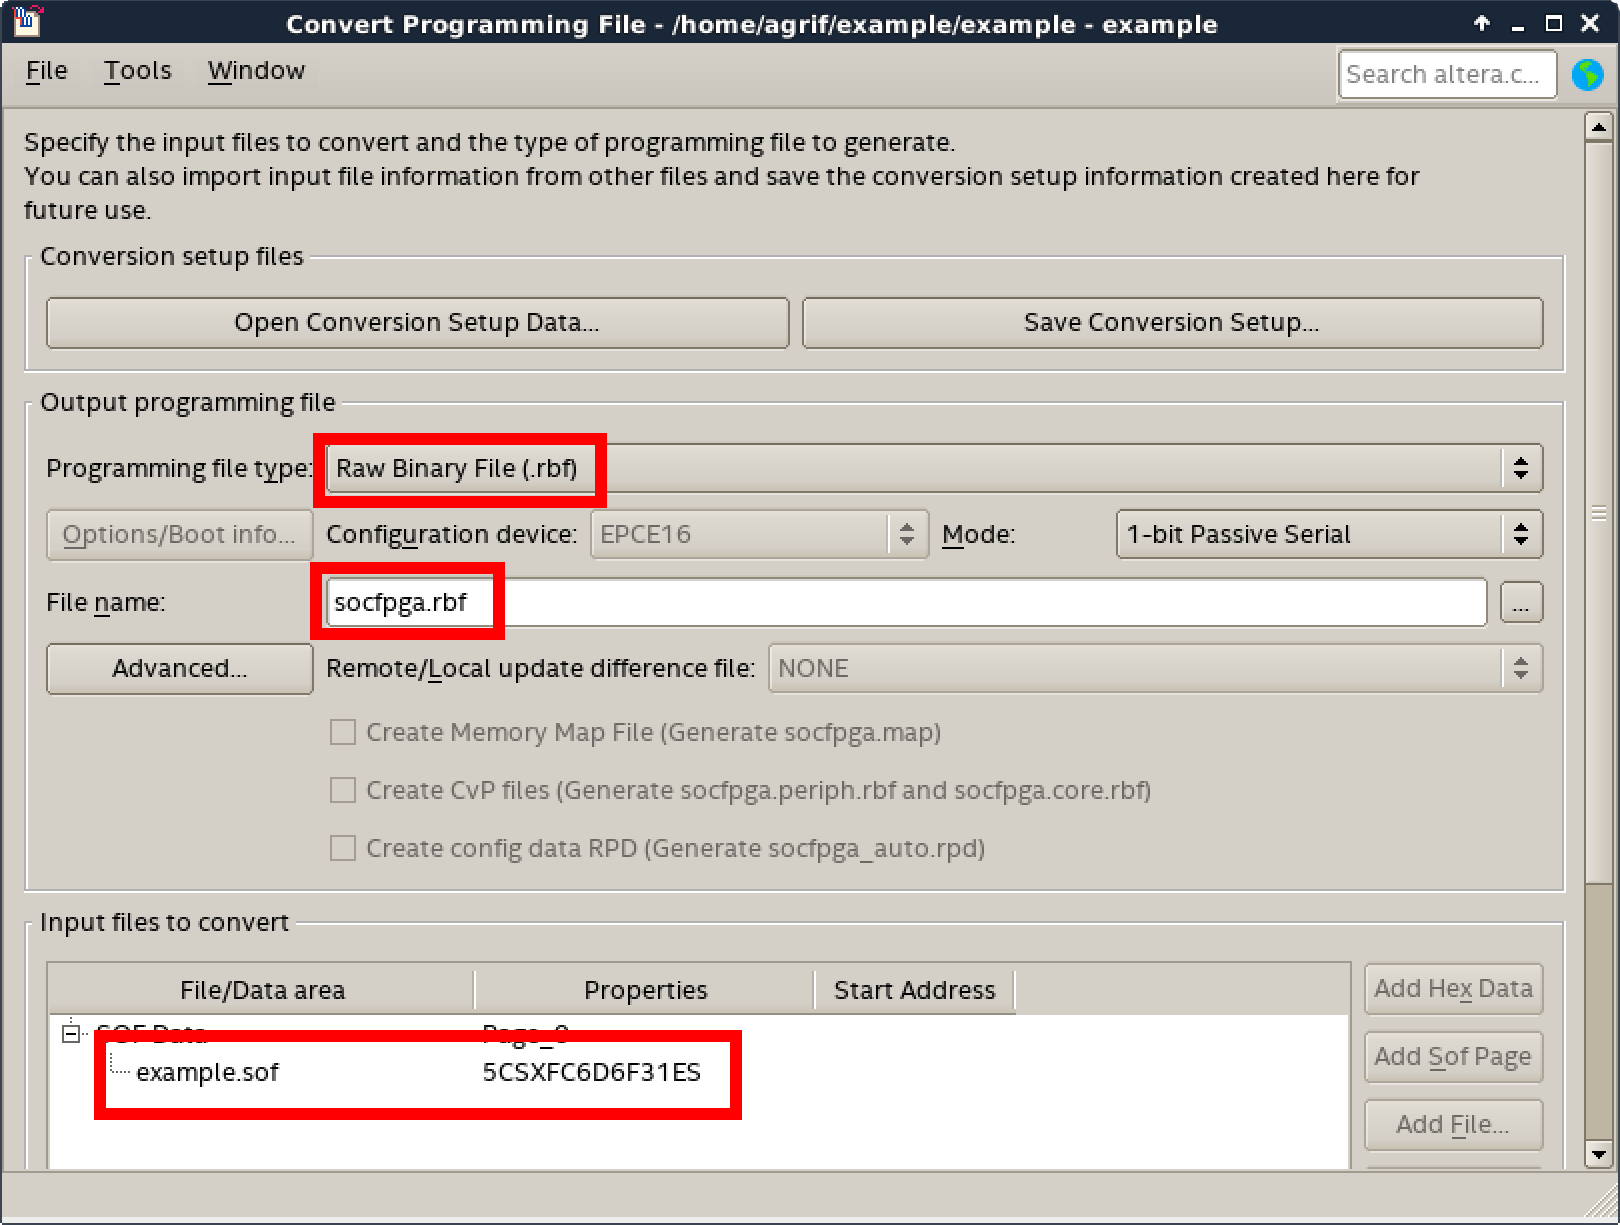
\includegraphics[width=8cm]{figures/rbf.png}
  \caption{Example settings for the Quartus programming file conversion window.}
  \label{fig:rbf}
\end{figure}

This file will program the FPGA, but now we need to provide Linux with
information about what sort of hardware the FPGA will provide. To do
this we will use the \texttt{dtbgen.py} script provided in the
example.

Remove the SD card from the SoCKit board, and put it back in your
computer. Copy the \directory{backup/socfpga.dtb} file off the SD card
somewhere handy. This file is an unmodified description of the
hardware on the board, that we will now modify to include the new
hardware provided by the FPGA. This \directory{backup} directory is
provided so that unmodified versions of these files are always
available.

Open up a terminal window, and navigate to the example project. There,
we will use \fnurl{Python 3}{https://www.python.org/} to run
\texttt{dtbgen.py}:
\begin{minted}{console}
  $ python3 dtbgen.py path/to/backup/socfpga.dtb \
    hps_system.sopcinfo -t dtb -o socfpga.dtb
\end{minted}

This will use information in \directory{hps\_system.sopcinfo}
(generated by Qsys) to modify the backup \directory{socfpga.dtb} to
create a new, modified \directory{socfpga.dtb}.

Armed with both these files, now copy \directory{socfpga.rbf} and
\directory{socfpga.dtb} to the SD card, and remove it and re-insert it
into the SoCKit board. Turn the board off then on again.

After a short pause, the board should load the RBF file, and you
should see the LEDs on the front of the board start to blink, counting
up in binary. If you see that, it worked!

\section{Using the Sampler and Player}

The SD card image we used comes loaded with a Linux kernel driver for
the Sampler and Player modules, as well as a Python module to
interface with them. We can test that out now. On the board's console,
launch Python:
\begin{minted}{console}
  $ python
  Python 2.7.9 (...)
  ...
  >>>
\end{minted}

To speak to the hardware now on the FPGA, we will use \texttt{numpy}
for dealing with data and a custom module \texttt{osuqlsp} for talking
to the Linux driver.
\begin{minted}{pycon}
  >>> import numpy, osuqlsp
\end{minted}

We will create a new \texttt{SPPair} object, which represents a
Sampler and Player linked together and running at the same time.
\begin{minted}{pycon}
  >>> sp = osuqlsp.SPPair('/dev/sampler0',
  ...       '/dev/player0')
\end{minted}

We can use this to play out data through the Player, while at the same
time reading in data through the Sampler. First, though, we need some
data. This hardware has been configured to deal with \num{1024}
discrete time steps, using \num{32} bits at each step. So we'll create
a \texttt{numpy} array of that size, full of zeros, and then set the
second bit on the $t = 1$ step to be \num{1}:
\begin{minted}{pycon}
  >>> data = numpy.zeros((1024, 32))
  >>> data[1, 2] = 1
  >>> data
\end{minted}
You should see Python print out a summary of our data.

Now, we can run it out through the Player, and see what results are
recorded on the Sampler:
\begin{minted}{pycon}
  >>> result = sp.run(data)
  >>> result
\end{minted}

You should see exactly the same data that was played in, delayed by
one time step. In this design, the Player is wired to turn on when the
Sampler does, but as this can only occur on a clock edge, in practice
the Player turns on one clock cycle after the Sampler, which leads to
this 1-cycle delay.

Data stored in \texttt{data[t, n]} will appear, one clock cycle
\texttt{t} at a time, inside the wire \texttt{player[n]} in the
Verilog design. And in the recorded data, \texttt{result[t, n]} will
be the value recorded on the wire \texttt{sampler[n]} on clock cycle
\texttt{t}. Since we have assigned \texttt{sampler} to equal
\texttt{player}, the data input to \texttt{sp.run} should match the
data output (except for the one cycle delay mentioned above).

A full tutorial on using Python is outside the scope of this guide,
but hopefully this will help you get started feeding data in to the
FPGA and reading data out.

You can press \keys{\ctrl + D} at the Python prompt to exit Python.

\section{Small Comforts}

This concludes the main part of the guide. However, there are some
small things you can do to make working on Linux on the board a little
bit more comfortable.

\subsection{Updating and Installing Software}

Debian comes with a built-in mechanism to update itself. To do so, you
can run:
\begin{minted}{console}
  $ sudo apt-get update
  $ sudo apt-get upgrade
\end{minted}

This will also pull in any fixes or updates to the Sampler/Player
software I may have released since the SD card image was made.

Debian also provides a ton of software pre-built for ARM chips like
the one on the SoCKit board. For example, to install \texttt{scipy}, a
scientific library for Python:
\begin{minted}{console}
  $ sudo apt-get install python-scipy
\end{minted}

\subsection{Creating a New User}

Your muscle memory might thank you for creating a new username and
password that is more familiar:
\begin{minted}{console}
  $ sudo adduser --add_extra_groups \
    --ingroup sudo <username>
  $ logout
\end{minted}

You can then log-in as the new user, and if you choose, delete the old
default user:
\begin{minted}{console}
  $ sudo deluser --remove-home sockit
\end{minted}

\subsection{Timezones and Locales}

The SD card is configured to use a UTC timezone, and generic United
States English locale. If you would prefer something different, run
one of:
\begin{minted}{console}
  $ sudo dpkg-reconfigure tzdata
  $ sudo dpkg-reconfigure locales
\end{minted}

\subsection{Setting a Hostname}

If you are working on a shared network, or using many SoCKit boards,
you might want to name them individually with something more unique
than \texttt{sockit}. You can use \texttt{nano}, a console-based
editor, to edit some files.

Movement is possible with the arrow keys. To write the changes and exit, press \keys{\ctrl + X} then \keys{Y}, then \keys{\enterwin} to confirm.

Edit \texttt{/etc/hostname} to replace \texttt{sockit} with your desired name:
\begin{minted}{console}
  $ sudo nano /etc/hostname
\end{minted}

Now, edit \texttt{/etc/hosts} and do the same
\begin{minted}{console}
  $ sudo nano /etc/hosts
\end{minted}

Finally, reboot to have the changes take effect:
\begin{minted}{console}
  $ sudo reboot
\end{minted}

\end{document}
